\section{Satellite galaxies around a massive central}

General code used in this exercise is:
\lstinputlisting[firstnumber=1, firstline=1, lastline=52]{Q1.py}



\subsection{a}

We have that
\begin{align*}
    \int\int\int_V n(x)\text{d}V &= \int\int\int n(x)x^2\sin(\phi)\text{d}\phi\text{d}\theta\text{d}x\\
    &=4\pi \int n(x)x^2\text{d}x\\
    &=4\pi \int x^2A\langle N_{sat}\rangle(\frac{x}{b})^{a-3}\exp{-(\frac{x}{b})^c}\text{d}x
    &=\langle N_{sat}\rangle.
\end{align*}
To solve for A, we find that
\begin{align*}
    4\pi A\int x^2(\frac{x}{b})^{a-3}\exp{-(\frac{x}{b})^c}\text{d}x &= 1\\
    A&=\frac{1}{4\pi \int x^2(\frac{x}{b})^{a-3}\exp{-(\frac{x}{b})^c}\text{d}x}.
\end{align*}
We are told to integrate from $x_{min}=0$ to $x_{max}=5$.
There is an integrable singularity at the limit $x=0$ (as dividing the integrand by zero is impossible), 
so an open method must be used to integrate this.
We choose to use the extended midpoint Romberg method (which is Richardson extrapolation applied to the midpoint rule).

The code used for this exercise is given here:
\lstinputlisting[firstnumber=56, firstline=56, lastline=95]{Q1.py}

The resulting value for A is:
\lstinputlisting[firstline=1, lastline=1]{output_Q1.txt}



\subsection{b}

We have made a random number generator consisting of a 64-bit XOR-shift generator followed by a 
multiple linear congruential generator, as mentioned in class. 
As parameters, we use $a_1=21$, $a_2=35$ and $a_3=4$ for the XOR shift, which are the parameters advised in class and the book.
For the MLCP we use $a=3741260$ and $m=4930622455819$, which are also numbers which are advised in the book. This results in a generator with
a period of $m-1$, because of which we can normalize the generated random integers to floats in the range (0,1) by dividing by $m-1$.
Testing the random number generator by having it generate 10000 random numbers results in the histogram shown in Figure \ref{fig:hist}.
As seen in the plot, the random numbers indeed result in quite a uniform distribution of numbers between 0 and 1.

The code for this exercise is given here:
\lstinputlisting[firstnumber=99, firstline=99, lastline=148]{Q1.py}

\begin{figure}[h!]
    \centering
    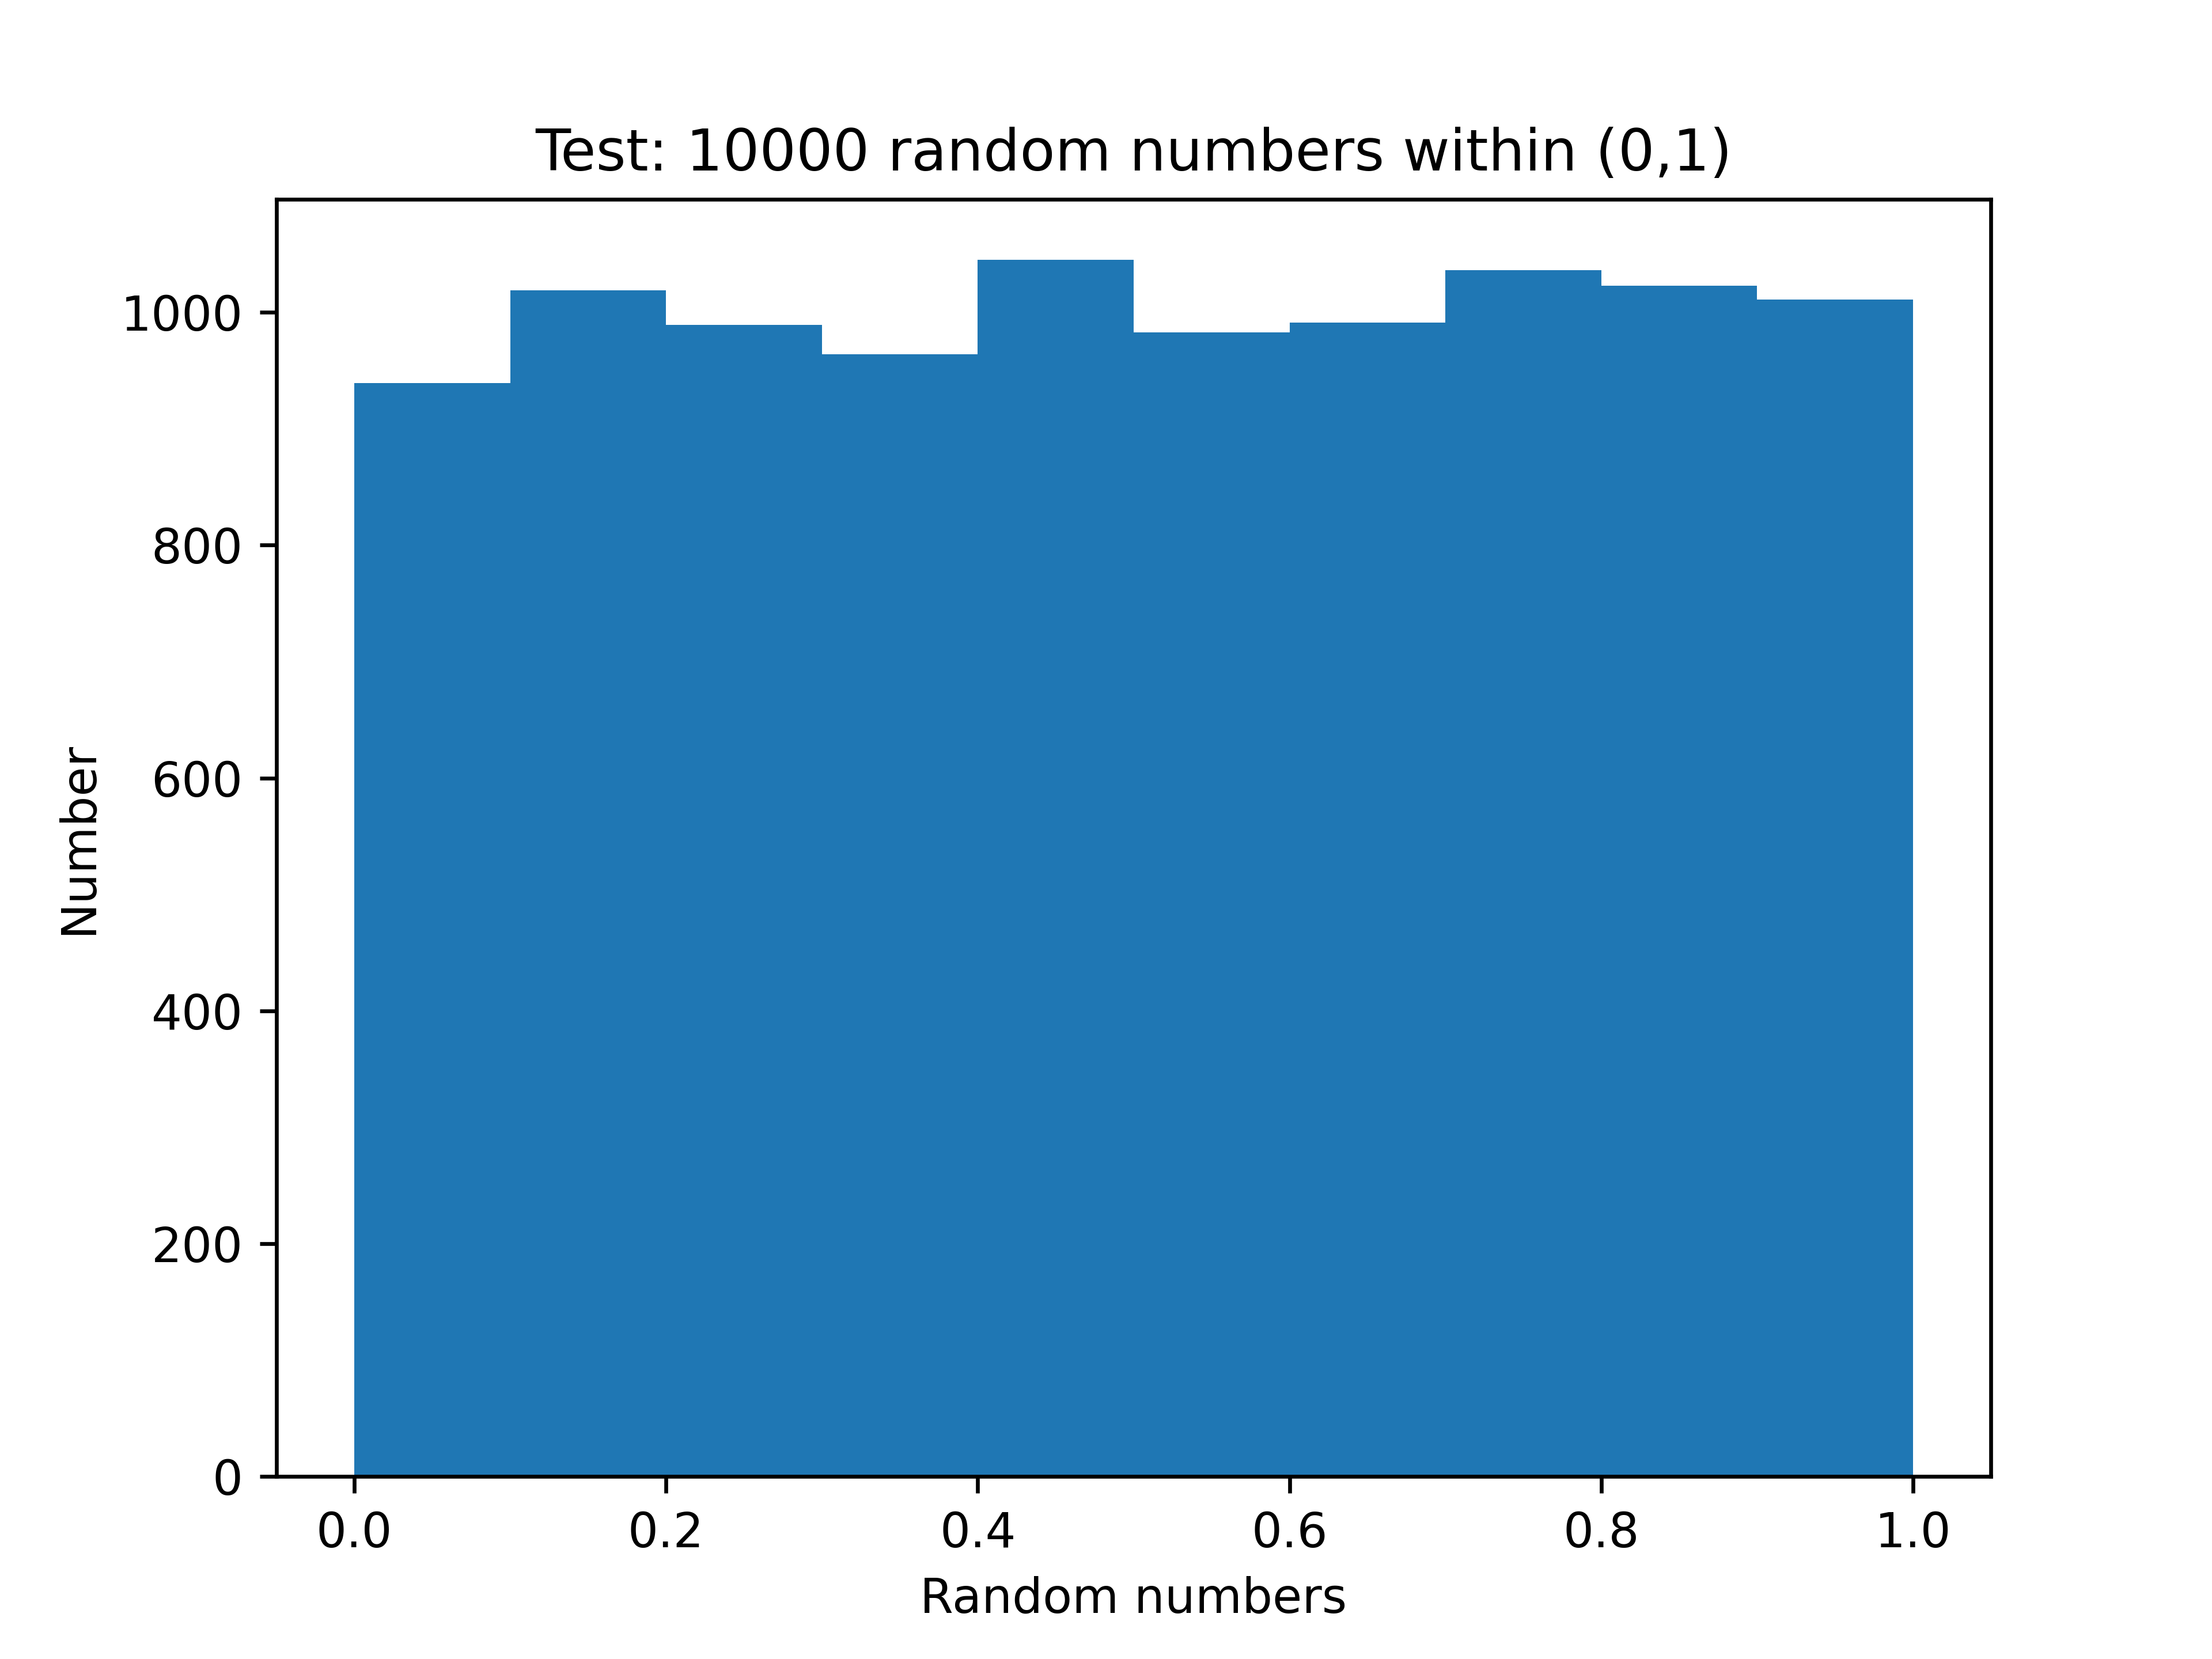
\includegraphics[width=0.9\linewidth]{./hist.png}
    \caption{A test of 10000 randomly generator numbers is shown. The distribution looks quite uniform, indicating that the RNG works as expected.}
    \label{fig:hist}
\end{figure}

We have that $N(x)\text{d}x$ is the number of galaxies in the infinitesimal range $[x,x+\text{d}x)$. To convert the number density $n(x)$
to $N(x)$, we have to integrate over $\phi$ and $\theta$. This gives that $N(x)=4\pi x^2n(x)$.

To sample from the probability distribution $p(x)=N(x)/N_{sat}$, we have implemented a rejection sampling algorithm.
We chose this algorithm, because it is relatively easy to implement and it turns out to run quite quickly
(even though it is a relatively slow method as it takes two random numbers and return less than 1 per draw).
The result of this sampling is shown in Figure \ref{fig:solb}.

\begin{figure}[h!]
    \centering
    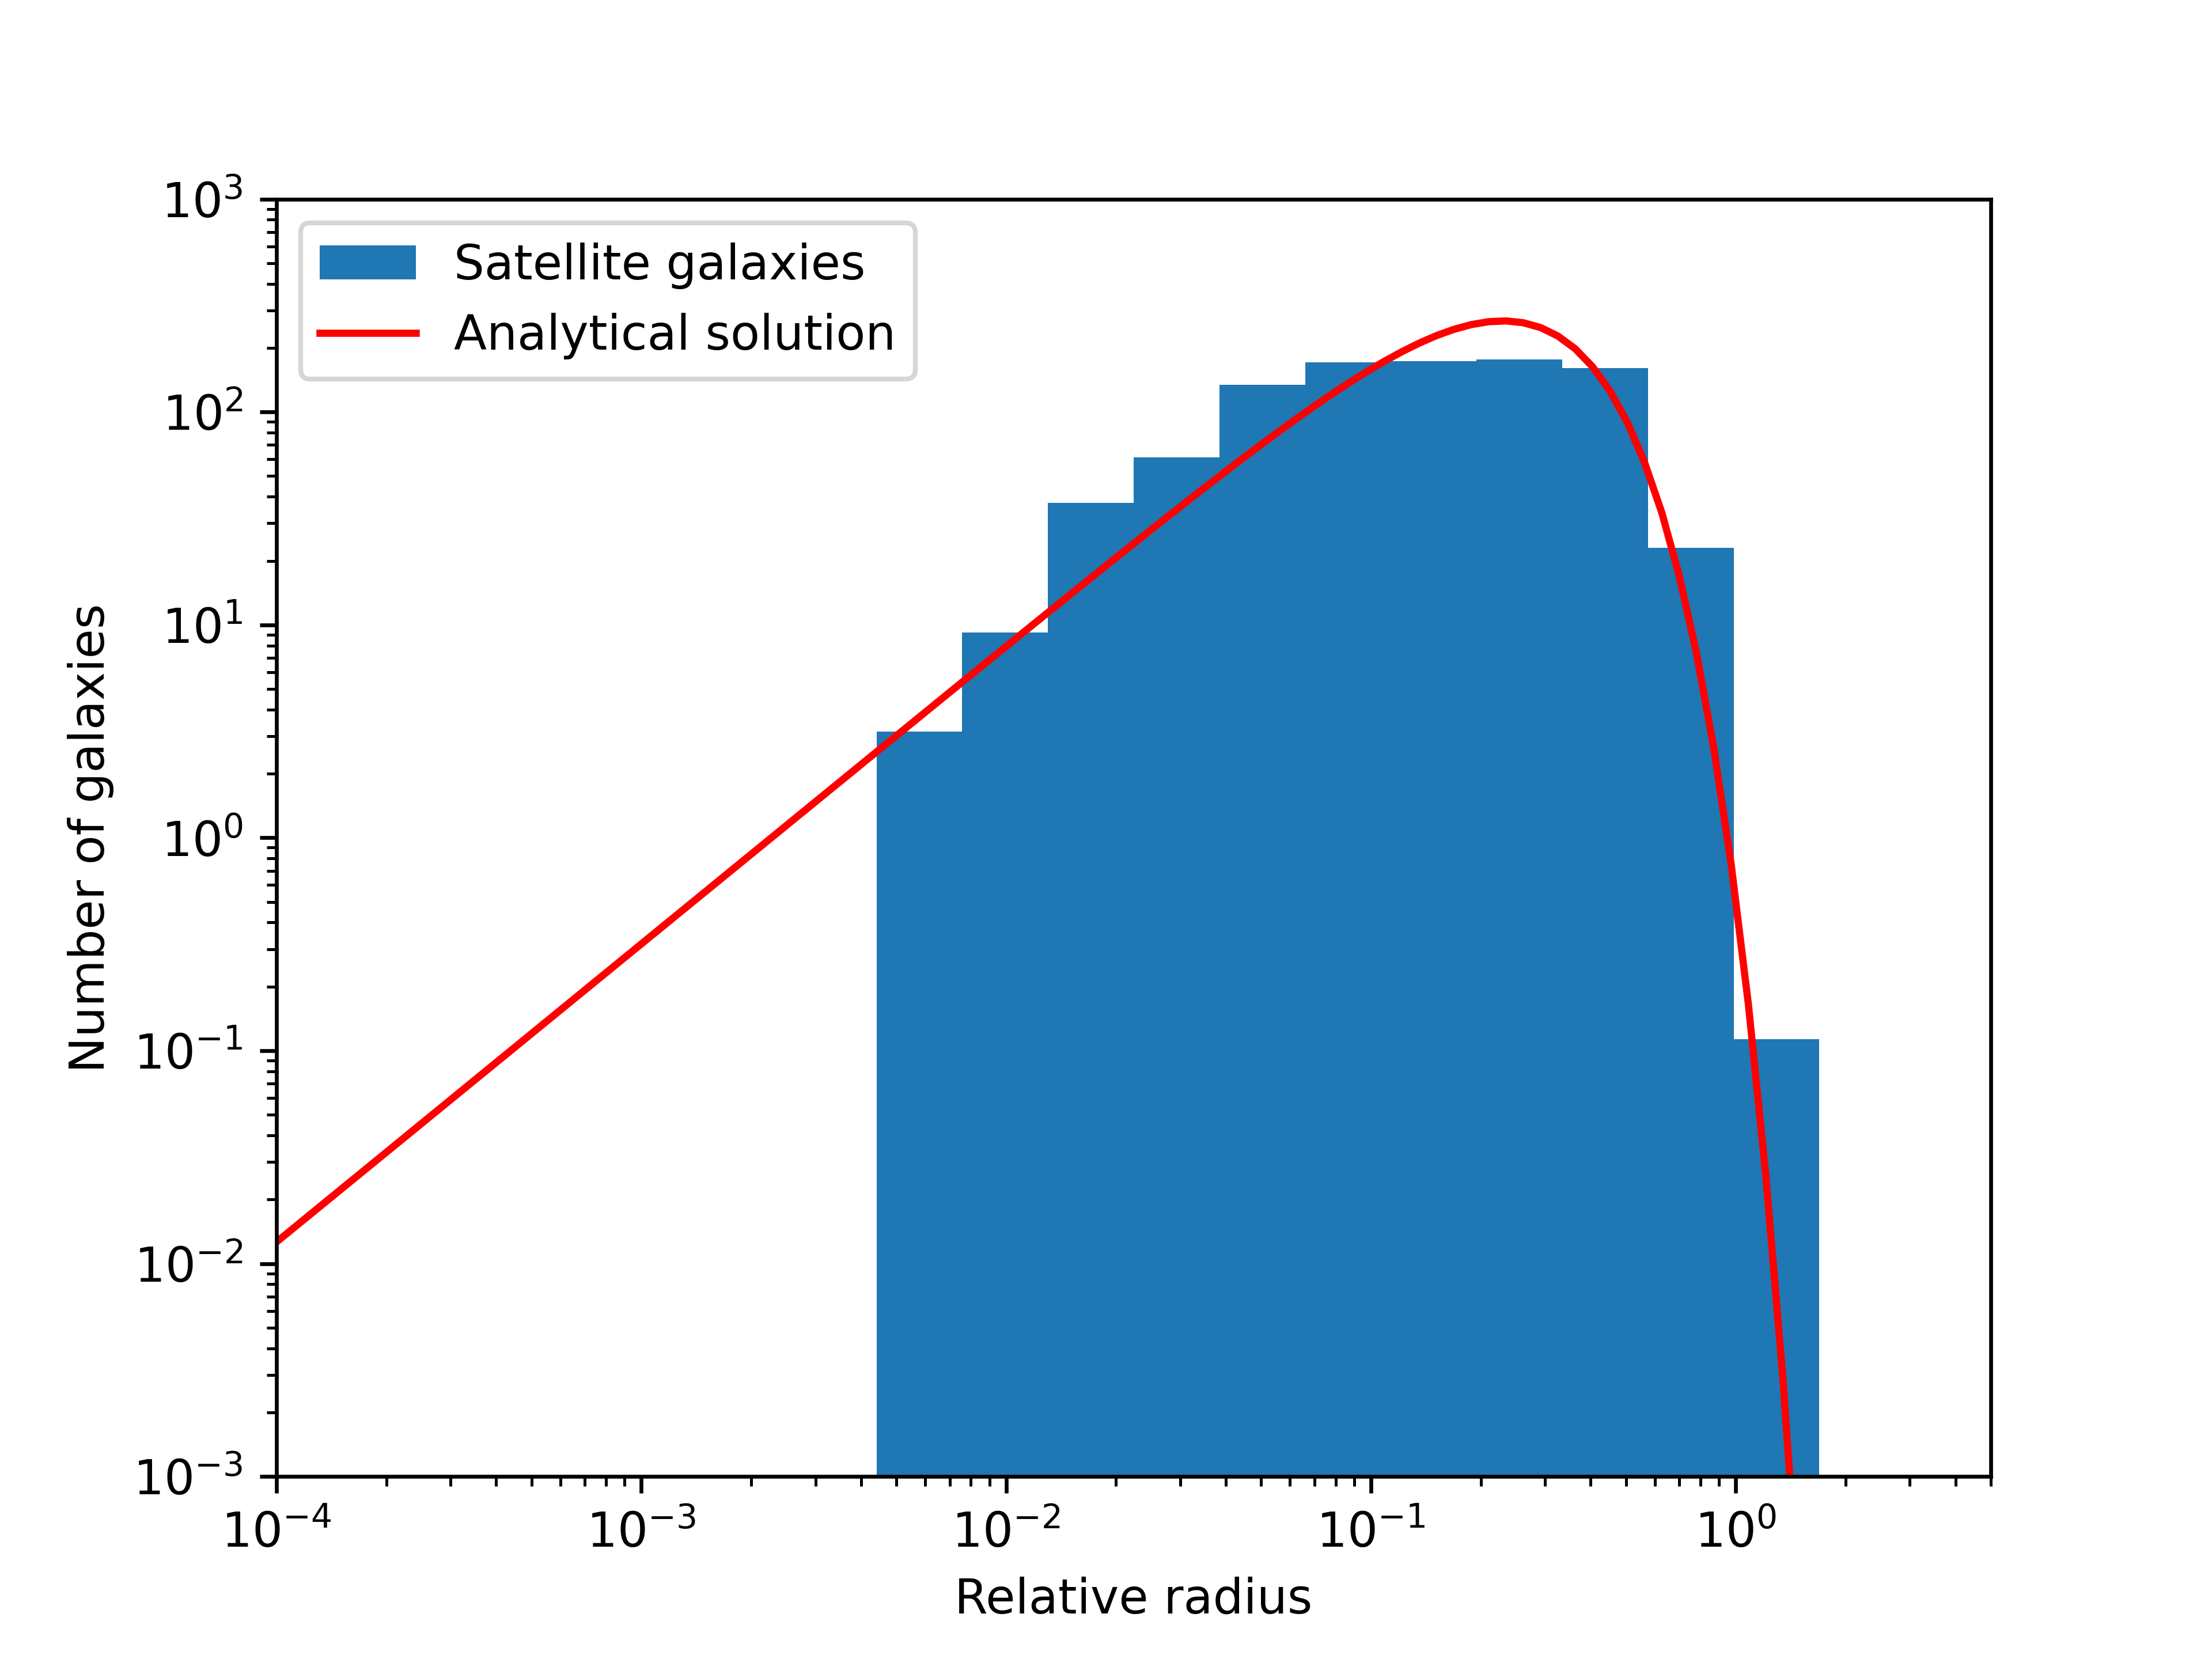
\includegraphics[width=0.9\linewidth]{./my_solution_1b.png}
    \caption{The histogram of 10000 sampled points from the distribution $p(x)$ are shown together with the analytical result for $N(x)$.
    The histogram is normalized both by the offset $10000/N_{sat}=100$ and by the width of the bins, in order to compare the shape with the
    analytical result. We see that the histogram follows the analytical shape very nicely for large $x$. However, for $x$ smaller than a certain
    threshold (about 0.005), the bins are all empty. This can probably be explained because our random number generator does not produce values
    which are as small.}
    \label{fig:solb}
\end{figure}



\subsection{c}

We select 100 random satellite galaxies from the 10000 random samples from (b) with a method that selects every galaxy with equal probability,
does not draw the same galaxy twice and does not reject any draw, by iteratively drawing one galaxy from the array, adding this to the new samples
and removing it from the original array, until we have 100 draws. Removing the drawn galaxies from the original array ensures we do not draw the same 
galaxy twice, such that we do not have to reject any draw. We draw a discrete index between 0 and the "length of the array-1=N-1" by sampling between (0,1) and scaling
multiplying by N to scale to (0, N), after which we take the floor such that the number is a random integer in [0, N-1].

We continue to sort the drawn galaxies using quicksort, as this method is the quickest method for the average typical case.
The result is shown in Figure \ref{fig:solc}, where the number of galaxies within a radius is plotted.

The code for this exercise is given here:
\lstinputlisting[firstnumber=152, firstline=152, lastline=226]{Q1.py}

\begin{figure}[h!]
    \centering
    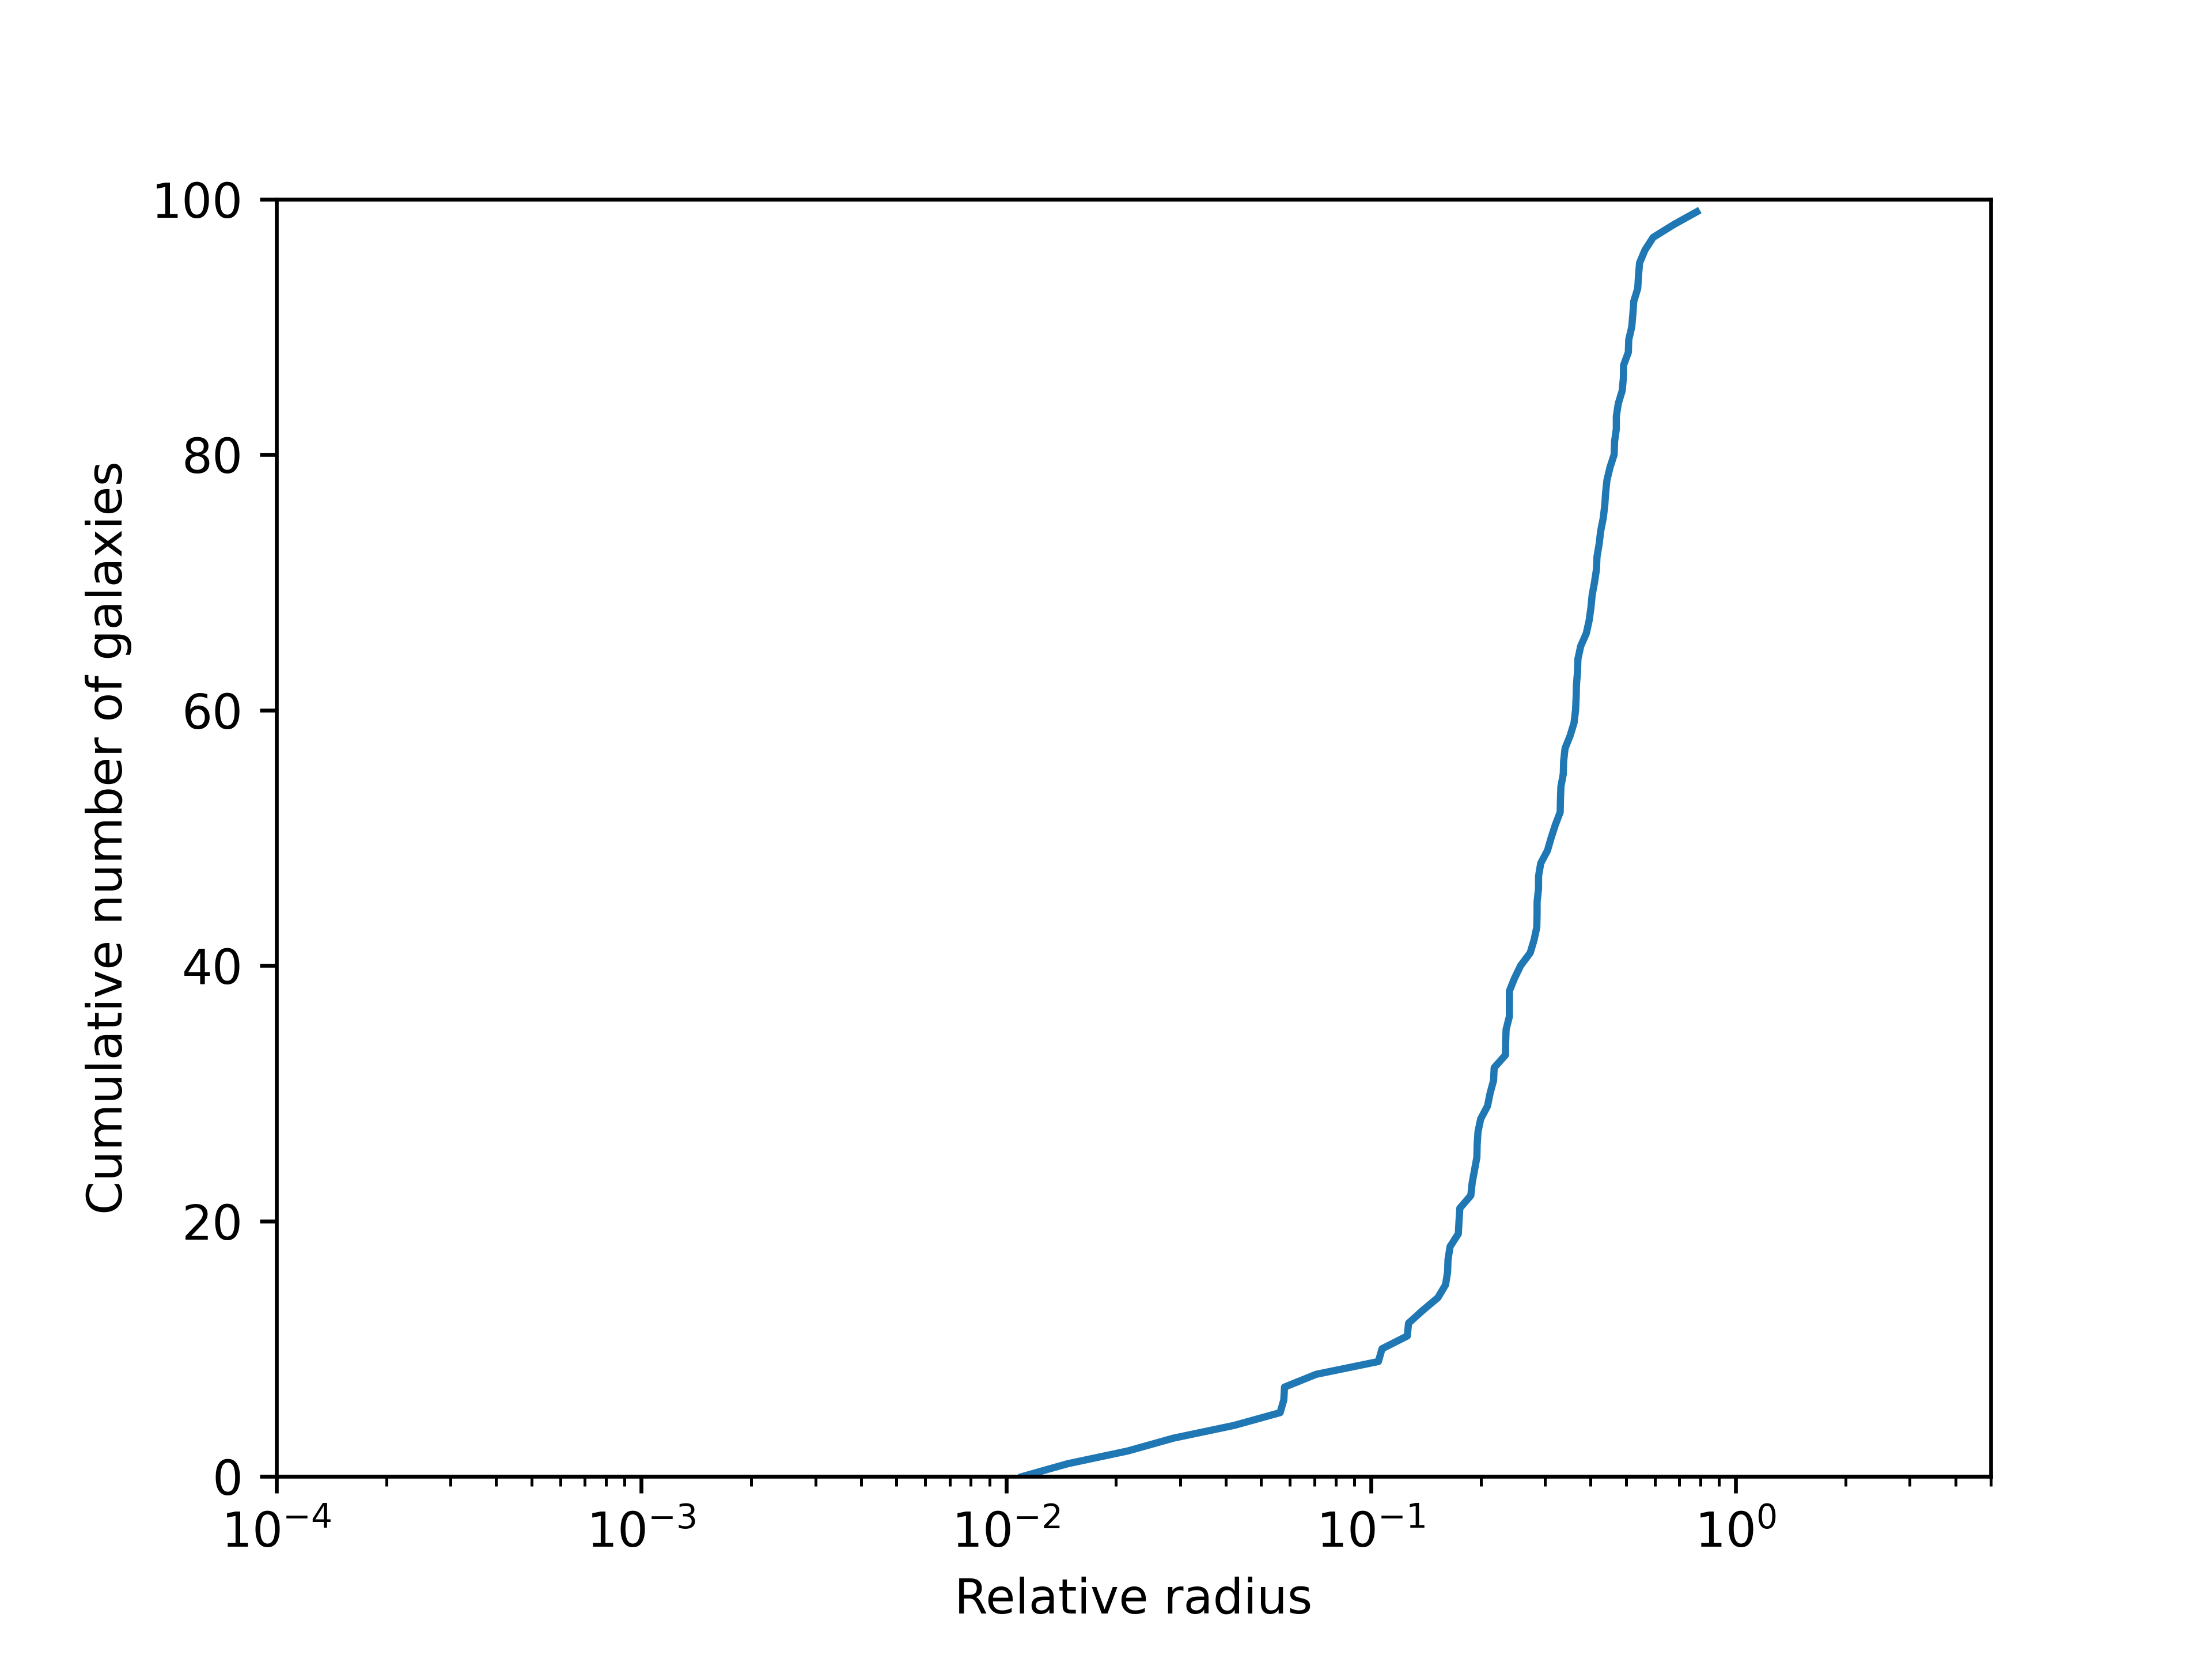
\includegraphics[width=0.9\linewidth]{./my_solution_1c.png}
    \caption{The number of galaxies within a radius is plotted (a cumulative distribution). It indeed looks like a cumulative distribution,
    which indicates that the samples are sorted correctly.}
    \label{fig:solc}
\end{figure}



\subsection{d}

To compute the derivative of $n$ at $x=1$ numerically we use Ridder's differentiation. The analytical result is given by taking the analytical derivative of $n$.

The used code is given here:
\lstinputlisting[firstnumber=230, firstline=230, lastline=263]{Q1.py}

The resulting values for the derivate are:
\lstinputlisting[firstline=2, lastline=3]{output_Q1.txt}
The analytical and numerical derivative are the same up to 13 significant digits.